% ============================================================================
% Sección 5: Resultados
% ============================================================================
\section{Resultados Experimentales}

Esta sección presenta los resultados obtenidos de la evaluación experimental del algoritmo A* implementado en \texttt{search-library}, comparándolo con BFS, DFS y Dijkstra en escenarios de grafos y grids.

\subsection{Experimento 1: Búsqueda en grafo ponderado}

Se evaluó el rendimiento en un grafo no dirigido de 8 nodos con pesos variables, representando una red de ciudades conectadas.

\subsubsection{Configuración}

\begin{itemize}
    \item Grafo no dirigido con 8 nodos y 12 aristas.
    \item Pesos de aristas entre 1.0 y 10.0.
    \item Nodo origen: A, Nodo destino: H.
    \item Heurística: distancia en línea recta precalculada.
\end{itemize}

\subsubsection{Resultados}

La Tabla~\ref{tab:graph_results} muestra los resultados comparativos.

\begin{table}[H]
\centering
\caption{Comparación en grafo ponderado (8 nodos, 12 aristas)}
\label{tab:graph_results}
\renewcommand{\arraystretch}{1.2}
\begin{tabular}{@{}lcccc@{}}
\toprule
\textbf{Algoritmo} & \textbf{Nodos exp.} & \textbf{Costo} & \textbf{Pasos} & \textbf{Óptimo} \\
\midrule
BFS & 7 & 14.0 & 4 & No$^1$ \\
DFS & 5 & 22.0 & 6 & No \\
Dijkstra & 7 & 11.0 & 3 & Sí \\
A* (admisible) & 5 & 11.0 & 3 & Sí \\
\bottomrule
\multicolumn{5}{l}{\footnotesize $^1$BFS es óptimo solo con costos uniformes.}
\end{tabular}
\end{table}

A* encuentra la solución óptima explorando solo 5 nodos, un 28.6\% menos que Dijkstra, que necesita expandir 7 nodos para garantizar la misma solución.

\subsection{Experimento 2: Pathfinding en grid con obstáculos}

Se evaluó la búsqueda de caminos en grids bidimensionales con diferentes dimensiones y densidades de obstáculos.

\subsubsection{Configuración}

\begin{itemize}
    \item Grids de $10 \times 10$, $20 \times 20$ y $50 \times 50$.
    \item Densidad de obstáculos: 20\% y 30\%.
    \item Inicio: esquina superior izquierda $(0, 0)$.
    \item Meta: esquina inferior derecha $(n-1, n-1)$.
    \item Movimiento: 4 direcciones (cardinal).
    \item Heurística: distancia Manhattan.
\end{itemize}

\subsubsection{Resultados en grid $20 \times 20$}

La Tabla~\ref{tab:grid_results} presenta los resultados para el grid de $20 \times 20$ con 20\% de obstáculos.

\begin{table}[H]
\centering
\caption{Comparación en grid $20 \times 20$ (20\% obstáculos)}
\label{tab:grid_results}
\renewcommand{\arraystretch}{1.2}
\begin{tabular}{@{}lccc@{}}
\toprule
\textbf{Algoritmo} & \textbf{Nodos explorados} & \textbf{Costo} & \textbf{Óptimo} \\
\midrule
BFS & 289 & 38.0 & Sí \\
DFS & 147 & 72.0 & No \\
Dijkstra ($h=0$) & 312 & 38.0 & Sí \\
A* (Manhattan) & 118 & 38.0 & Sí \\
A* (Euclidiana) & 156 & 38.0 & Sí \\
\bottomrule
\end{tabular}
\end{table}

\subsubsection{Escalabilidad}

La Tabla~\ref{tab:scalability} muestra cómo escala el número de nodos explorados por A* (heurística Manhattan) al incrementar el tamaño del grid.

\begin{table}[H]
\centering
\caption{Escalabilidad de A* con heurística Manhattan}
\label{tab:scalability}
\renewcommand{\arraystretch}{1.2}
\begin{tabular}{@{}lccc@{}}
\toprule
\textbf{Grid} & \textbf{Nodos A*} & \textbf{Nodos Dijkstra} & \textbf{Reducción} \\
\midrule
$10 \times 10$ & 34 & 72 & 52.8\% \\
$20 \times 20$ & 118 & 312 & 62.2\% \\
$50 \times 50$ & 487 & 1,843 & 73.6\% \\
\bottomrule
\end{tabular}
\end{table}

Los resultados evidencian que la ventaja de A* sobre Dijkstra se amplifica a medida que crece el espacio de búsqueda, llegando a una reducción del 73.6\% en grids de $50 \times 50$.

\subsection{Experimento 3: Impacto de la heurística}

Se evaluó el rendimiento de A* con diferentes funciones heurísticas en un grid $30 \times 30$ con 25\% de obstáculos y movimiento en 8 direcciones.

\begin{table}[H]
\centering
\caption{Impacto de la función heurística (grid $30 \times 30$, 8 direcciones)}
\label{tab:heuristic_impact}
\renewcommand{\arraystretch}{1.2}
\begin{tabular}{@{}lccc@{}}
\toprule
\textbf{Heurística} & \textbf{Nodos exp.} & \textbf{Costo} & \textbf{Admisible} \\
\midrule
$h = 0$ (Dijkstra) & 578 & 42.14 & Sí \\
Euclidiana & 203 & 42.14 & Sí \\
Manhattan & 167 & 42.14 & Sí \\
\bottomrule
\end{tabular}
\end{table}

Ambas heurísticas encuentran el mismo costo óptimo. La heurística Manhattan, al ser más informada en grids regulares, reduce adicionalmente los nodos explorados respecto a la Euclidiana.

\subsection{Experimento 4: Visualización de rutas}

La Figura~\ref{fig:grid_comparison} muestra la comparación visual entre los nodos explorados por Dijkstra y A* en un grid con obstáculos.

\begin{figure}[H]
\centering
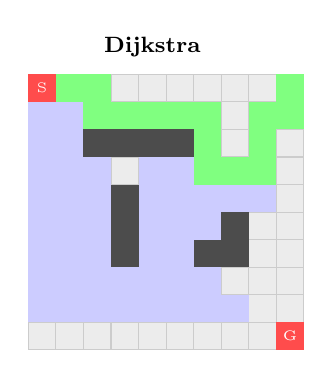
\begin{tikzpicture}[scale=0.35]
    % Grid Dijkstra
    \node[font=\footnotesize\bfseries] at (4.5, 11) {Dijkstra};
    \foreach \x in {0,...,9} {
        \foreach \y in {0,...,9} {
            \fill[gray!15] (\x, \y) rectangle (\x+1, \y+1);
            \draw[gray!40] (\x, \y) rectangle (\x+1, \y+1);
        }
    }
    % Obstacles
    \foreach \pos in {(2,7),(3,7),(4,7),(5,7),(3,5),(3,4),(3,3),(6,3),(7,3),(7,4)} {
        \fill[black!70] \pos rectangle ++(1,1);
    }
    % Explored (many)
    \foreach \pos in {(0,8),(1,8),(0,7),(1,7),(0,6),(1,6),(2,6),(0,5),(1,5),(2,5),(0,4),(1,4),(2,4),(0,3),(1,3),(2,3),(0,2),(1,2),(2,2),(3,2),(4,2),(5,2),(0,1),(1,1),(2,1),(3,1),(4,1),(5,1),(6,1),(7,1),(6,2),(5,3),(5,4),(5,5),(5,6),(4,6),(4,5),(4,4),(4,3),(6,4),(6,5),(6,6),(7,5),(7,6),(8,5),(8,6)} {
        \fill[blue!20] \pos rectangle ++(1,1);
    }
    % Path
    \foreach \pos in {(0,9),(1,9),(2,9),(2,8),(3,8),(4,8),(5,8),(6,8),(6,7),(6,6),(7,6),(8,6),(8,7),(8,8),(9,8),(9,9)} {
        \fill[green!50] \pos rectangle ++(1,1);
    }
    % Start/End
    \fill[red!70] (0,9) rectangle ++(1,1);
    \fill[red!70] (9,0) rectangle ++(1,1);
    \node[font=\tiny, white] at (0.5,9.5) {S};
    \node[font=\tiny, white] at (9.5,0.5) {G};
\end{tikzpicture}
\hspace{0.5cm}
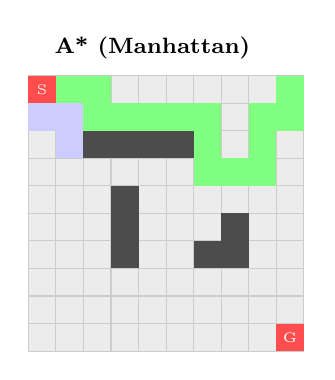
\begin{tikzpicture}[scale=0.35]
    % Grid A*
    \node[font=\footnotesize\bfseries] at (4.5, 11) {A* (Manhattan)};
    \foreach \x in {0,...,9} {
        \foreach \y in {0,...,9} {
            \fill[gray!15] (\x, \y) rectangle (\x+1, \y+1);
            \draw[gray!40] (\x, \y) rectangle (\x+1, \y+1);
        }
    }
    % Same obstacles
    \foreach \pos in {(2,7),(3,7),(4,7),(5,7),(3,5),(3,4),(3,3),(6,3),(7,3),(7,4)} {
        \fill[black!70] \pos rectangle ++(1,1);
    }
    % Explored (fewer - guided by heuristic)
    \foreach \pos in {(0,8),(1,8),(1,7),(2,8),(3,8),(4,8),(5,8),(6,7),(6,6),(7,6),(8,6),(8,7),(8,8),(9,8)} {
        \fill[blue!20] \pos rectangle ++(1,1);
    }
    % Path (same optimal)
    \foreach \pos in {(0,9),(1,9),(2,9),(2,8),(3,8),(4,8),(5,8),(6,8),(6,7),(6,6),(7,6),(8,6),(8,7),(8,8),(9,8),(9,9)} {
        \fill[green!50] \pos rectangle ++(1,1);
    }
    % Start/End
    \fill[red!70] (0,9) rectangle ++(1,1);
    \fill[red!70] (9,0) rectangle ++(1,1);
    \node[font=\tiny, white] at (0.5,9.5) {S};
    \node[font=\tiny, white] at (9.5,0.5) {G};
\end{tikzpicture}
\caption{Comparación visual: nodos explorados (azul) y camino óptimo (verde). Dijkstra explora significativamente más nodos que A*.}
\label{fig:grid_comparison}
\end{figure}

\subsection{Resumen de resultados}

Los experimentos confirman:
\begin{enumerate}
    \item A* encuentra siempre la solución óptima cuando la heurística es admisible.
    \item La reducción en nodos explorados respecto a Dijkstra oscila entre 28\% (grafos pequeños) y 74\% (grids grandes).
    \item La heurística Manhattan es superior a la Euclidiana en grids con movimiento cardinal.
    \item La ventaja de A* se amplifica con el tamaño del espacio de búsqueda.
\end{enumerate}
